\documentclass[12pt]{exam}

\usepackage[margin=0.5in]{geometry}
\usepackage{amsmath,amssymb}
\usepackage{tikz,soul}
\usepackage{diagbox}
\usetikzlibrary{arrows,automata,positioning}

\newcommand{\ds}{\displaystyle}
\newcommand{\bs}{\backslash}
\newcommand{\on}{\operatorname}
\newcommand{\R}{\mathbb{R}}
\newcommand{\Z}{\mathbb{Z}}
\newcommand{\N}{\mathbb{N}}

\begin{document}
\pagestyle{empty}
\subsubsection*{Homework 3 - Computer Science 461 \hfill Name: \underline{\hspace*{2in}}}

\textit{Due Monday, February 3.} % You can e-mail your code for the computer programming problems to me at }\verb|blins@hsc.edu|.

\begin{questions}

\question Consider the DFA shown below.  


\begin{minipage}{0.46\textwidth}
\small
\begin{parts}
\part What are the sets $Q$, $\Sigma$, and $F$ in the formal description $(Q,\Sigma,\delta,q,F)$ of this machine?
\vspace*{1in}

\part What sequence of states does the machine go through on the input \verb|aabbaa|?  Does the machine accept \verb|aabbaa|? 
\vspace*{0.8in}
\end{parts}
\end{minipage}
\hfill
%second column (no space between first and second column!)
\begin{minipage}{0.4\textwidth}
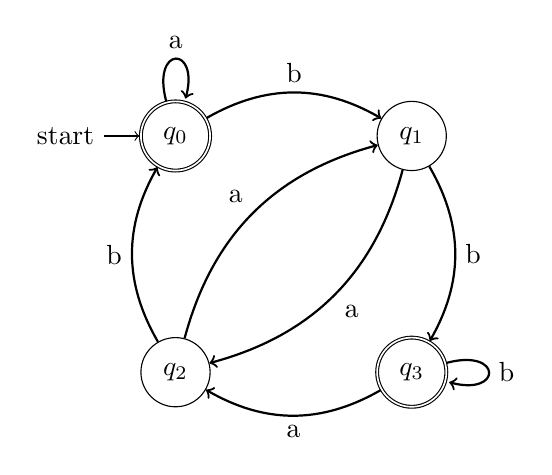
\begin{tikzpicture}[node distance=3cm,auto]
  %\tikzstyle{every state}=[fill={rgb:black,1;white,10}]

  \node[state,initial,accepting] (q_0)        {$q_0$};
  \node[state]           (q_1) [right of=q_0] {$q_1$};
  \node[state]           (q_2) [below of=q_0] {$q_2$};
  \node[state,accepting] (q_3) [right of=q_2] {$q_3$};
  \path[thick,->]
  (q_0) edge [bend left] node {b} (q_1)
        edge [loop above]  node {a} ()
  (q_1) edge [bend left] node {b} (q_3)
        edge [bend left] node {a} (q_2)
  (q_2) edge [bend left] node {a} (q_1)
        edge [bend left] node {b} (q_0)
  (q_3) edge [bend left] node {a} (q_2)
        edge [loop right] node {b} ();
\end{tikzpicture}
\vspace*{1.0in}
\end{minipage}


\question Design a DFA that outputs 1 if and only if the input length is divisible by 3. Draw a state diagram for you answer.
\vfill
\vfill

\question Design a DFA that outputs 1 if and only if the input begins with 01 and ends with 01.  Draw a state diagram for your answer. 
\vfill
\vfill

\newpage
\question Construct an NFA with three states that accepts a string in $\{0,1\}^*$ iff it ends in 00.  
\vfill
\vfill

\question Find a DFA that is equivalent to the NFA shown below. 
\begin{flushright}
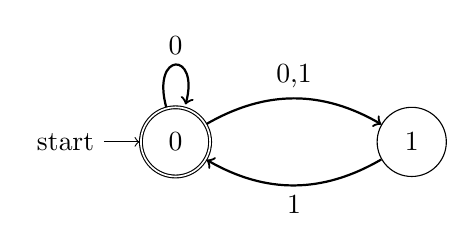
\begin{tikzpicture}[node distance=3cm,auto]
  %\tikzstyle{every state}=[fill={rgb:black,1;white,10}]

  \node[state,initial,accepting] (q_0)        {$0$};
  \node[state]           (q_1) [right of=q_0] {$1$};
  \path[thick,->]
  (q_0) edge [bend left] node {0,1} (q_1)
        edge [loop above]  node {0} ()
  (q_1) edge [bend left] node {1} (q_0);
\end{tikzpicture}
\end{flushright}
\vfill

\question Consider a DFA with states $Q = \{0,1,2\}$, alphabet $\Sigma = \{0,1\}$, initial state $q_0 = 0$, and accepting states $F = \{0, 1\}$.  The transition function is shown in the table below. Write a computer program that takes a string in $\Sigma^*$ as input and prints each state the DFA enters as it goes through the input string. Your program should also return 1 if the DFA accepts the string, otherwise return 0.  %Test your program on the string 1100111000.

\begin{flushright}
\begin{tabular}{c|cc} 
\backslashbox{q}{$\sigma$} & 0 & 1 \\ \hline
0 & 1 & 1 \\ 1 & 0 & 2 \\
2 & 0 & 0
\end{tabular}
\end{flushright}
\vfill

\end{questions}
\end{document}
